\subsection{Validation of the methodology}

\subsection{Testing on a real scenario}
\label{sec:real}

%As stated in Secs.~\ref{sec:equipment}~and~\ref{sec:limitations}, a partial point cloud
%of a segmented object is required in order to get observation points for the initial
%surface estimation and speed up the shape modeling.
%\citet[Sec.~III.A]{Hudson2012Endtoend}  provides  good   candidate algorithms  for  object
%segmentation  that are  well oriented  to  object grasp,  manipulation, and  for
%our  purposes, exploration.  In fact,  the  combination of  their ``Table  Plane
%Estimation''  with their  ``Volume-Based  Segmentation''  yields the  ubiquituos
%tabletop object segmentation \citep{TabletopObjectDetector}. However, to improve
%the  rechability  of the  exploration,  we  prefer to  hold  the  object in  one
%hand-arm system and explore with the other, as described in Sec.~\ref{sec:scope}.
%\todo[]{Descrition in section 3 is missing. Also should point to the subsection, not the section.}
%Thus,  our selected  approach  for  object segmentation  is  simpler than  those
%approaches.  The  difficulties are  in  measuring  the  configuration of  a  soft
%and  adaptable  hand, like the Pisa/IIT SoftHand,
%\todo[]{I think we should cite some softhand paper here.}
%that  keeps  the  object  in  position  to  filter  out
%the  points  belonging  to  the  hand-arm system.  For  this  purpose,  one  can
%rely in  body-type measurements  instead of  traditional encoders,  as described
%in~\citet{Santaera2015Lowcost}.

We assume that the robot holds the object in its left hand. This allows the robot to move the object in a position where a snapshot of the object can be taken from the RGB-D camera disposed on its chest. \todo[]{we should put here a picture of Vito observing the object and what it is visible in simulation}
The acquired point cloud is an incomplete, noisy observation of the object, but it also likely contains other elements like, for example, the robot's hand-arm system as well as part of the background. 

Our propose solution to isolate the object's point cloud is to firstly utilise the robot's proprioception to remove the parts of the point cloud that most likely belong to the robot's body. However, measuring  the  configuration of  a  soft and  adaptable hand, like the Pisa/IIT SoftHand, is a challenging problem. For this purpose, we rely on a similar solution proposed by~\citet{Santaera2015Lowcost}; a sensorised glove which allows us to estimate the kinematic configuration of the soft hand at any time.

Once the hand-arm  system pose is measured, then
some   passthrough filters with slightly  scaled bounding boxes of  the robot
geometry  are used  to obtain  a  point cloud  of  the object  isolated from  the
robot. The scaling factor $\kappa$ is used to account for any incertainties that might
be present in the robot state or in the point cloud measurements. 
By slightly enlarging the robot bounding boxes we make sure that the object is correctly
separated from it, at the cost of losing some object points on the hand-object edge.

A further box filter is then applied to isolate the object from the rest of the scene,
thus obtaining a segmented object point cloud. 
Finally the obtained point cloud is further resampled to reduce the overall point
density, mantaining the object geometrical properties, while at the same time
improving Gaussian Process computation speed. 
\todo[]{Perhaps voxel grid description can be omitted}

This last downsampling step is performed with a Voxel Grid Filter, which, after
building a grid of voxels on top of the point cloud, it
substitutes all points in a voxel with their centroid, thus reducing the total number of 
points, while maintaining the object geometrical properties intact. The final desired
point cloud resolution can be controlled with $\delta$ parameter, which is just the edge length of each voxel.
Fig.~\ref{fig:in-hand-segmentation} shows the procedure applied to a real scene,
while  Algorithm~\ref{alg:in-hand-segmentation} resumes  the whole  procedure in
the pseudo-code.

% \begin{algorithm}[h]
%     \textbf{$\mathcal{O} \leftarrow$ \textsc{segmentInHand}}($\mathcal{P}$, $\mathcal{R}$, $\kappa$, $\delta$)\\ %functionname
% \LinesNumbered
% \DontPrintSemicolon
% \SetAlgoVlined \SetKwInOut{Input}{input} \SetKwInOut{Output}{output}
% \Input{The complete scene point cloud, $\mathcal{P}$, the robot model, $\mathcal{R}$, its visual geometry inflation factor, $\kappa$, and the downsampling resolution, $\delta$.}
% \Output{The segmented object point cloud, isolated from the scene, $\mathcal{O}$.}
%   $\mathbf{r} \leftarrow$\textsc{robotState}($\mathcal{R}$) \\
%   $\mathcal{B} \leftarrow$\textsc{boundingBoxes}($\mathcal{R}$, $\mathbf{r}$, $\kappa$) \\
%   $\mathcal{O^\prime} \leftarrow$\textsc{passtroughFilters}($\mathcal{P}$, $\mathcal{B}$) \\
%   $\mathcal{O} \leftarrow$\textsc{downsampleFilter}($\mathcal{O^\prime}$, $\delta$) \\
%   \Return{$\mathcal{O}$}
% \caption{In-hand object segmentation.} \label{alg:in-hand-segmentation}
% \end{algorithm}

The \textsc{robotState}($\cdot$) method retrievs istantaneous joint states
of the whole hand-arm system ($\mathbf{r}$), which is used by \textsc{boundingBoxes($\cdot$)} to compute robot bounding boxes ($\mathcal{B}$)
from its geometrical properties, known by the robot model ($\mathcal{R}$).

\textsc{passtroughFilters}($\cdot$) repeatedly performs filters to remove
all points found inside the hand-arm system bounding boxes, obtaining $\mathcal{O^\prime}$.
That is finally resampled with the desired resolution ($\delta$) 
to obtain the final segmented object ($\mathcal{O}$), in \textsc{downsampleFilter}($\cdot$) function.

\todo[inline]{rewording-removal?}

To notice that our propose approach does not need to have an initial point cloud to start the exploration procedure. A GP could be instantiated with no input data and successively refined by adding to the model only the haptic clues. However the GP inference process will be affected especially in the earlier stages of the procedure.   
%It is worth noting, that this procedure is here also to show how visual and tactile
%data might  be merged into a  single shape model.
%But,  as a matter of  fact, the
%initial training  point set  can be  empty and the whole shape modeling could be 
%started  by simply  probing naively towards the gripper.

\begin{figure}
\centering
  \mbox{
  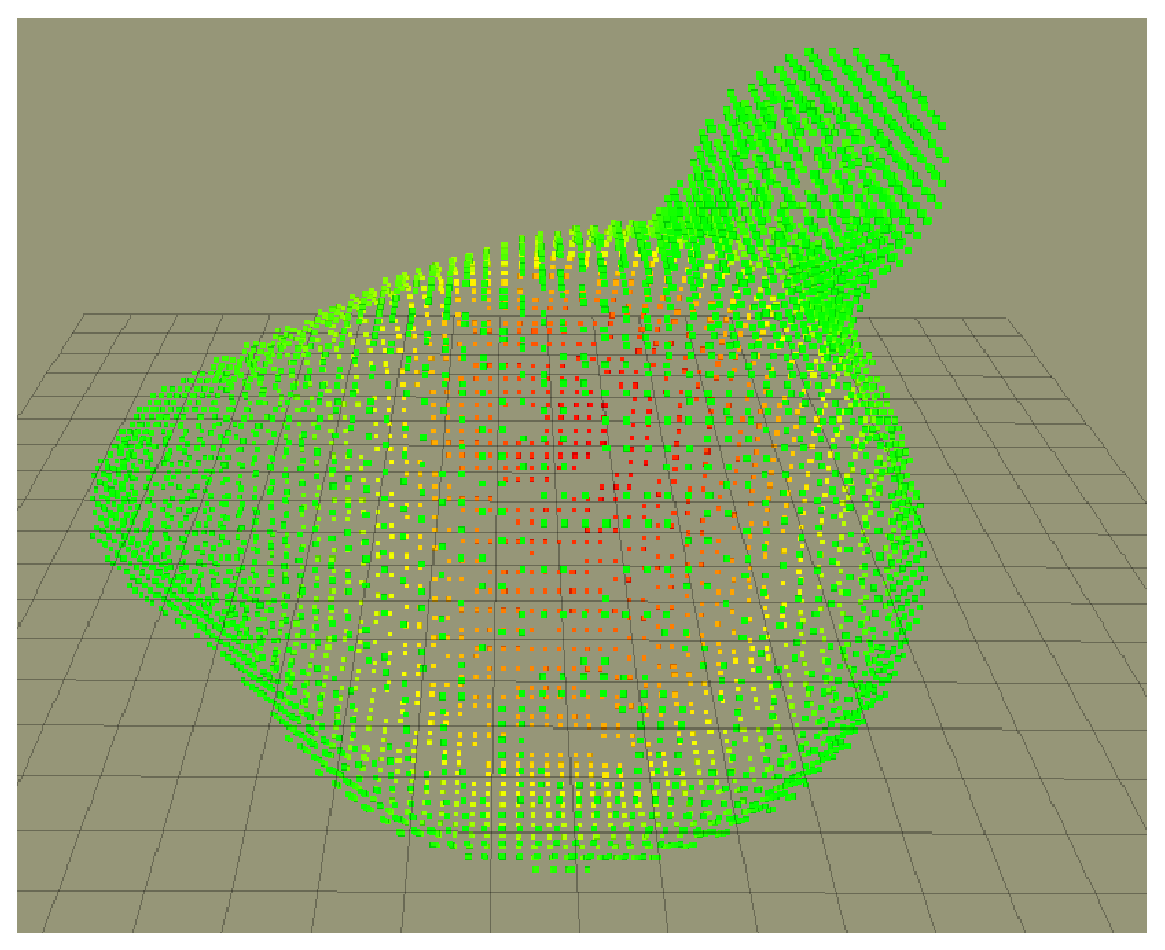
\includegraphics[width=0.45\linewidth]{example.eps}
  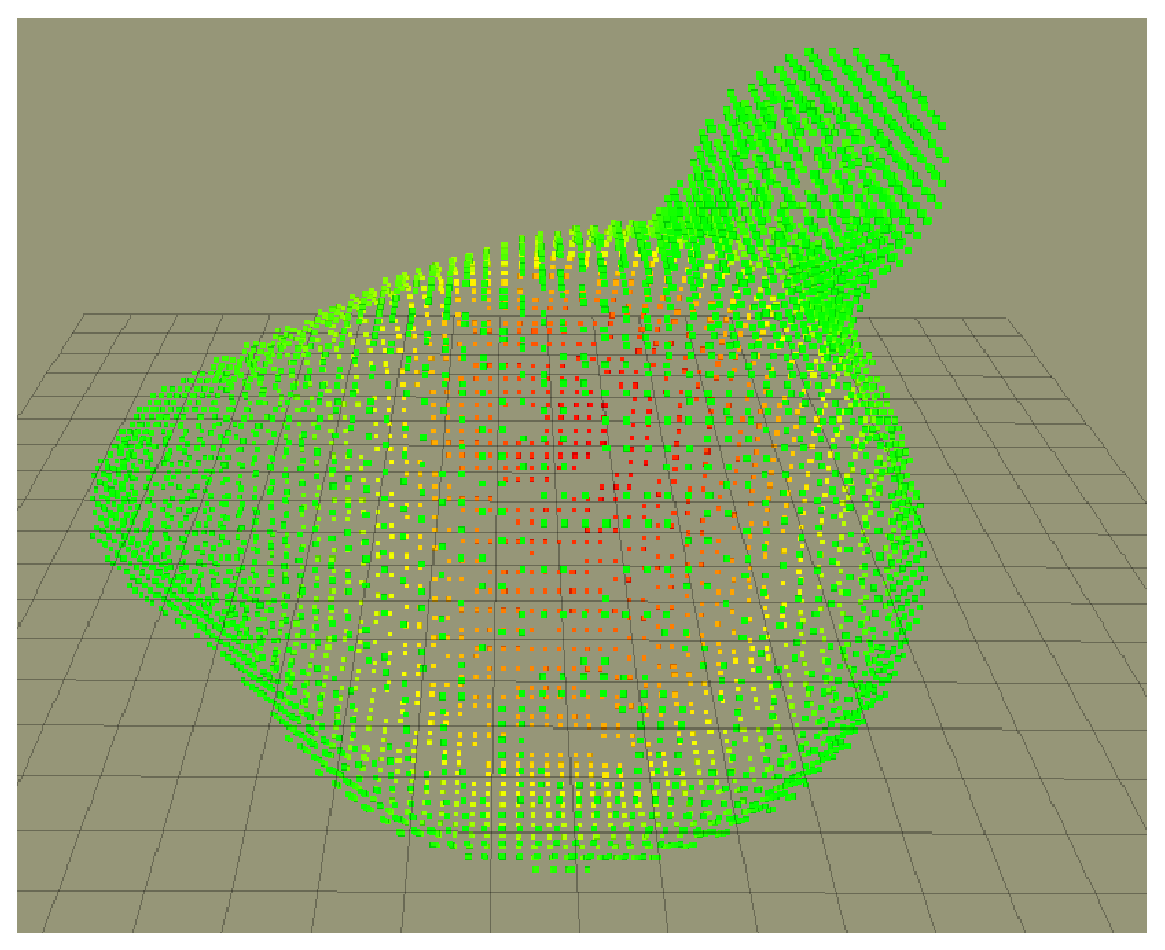
\includegraphics[width=0.45\linewidth]{example.eps}
  }
  \caption{A picture of the in-hand object segmentation using a soft-adaptive hand on a 7-dof arm in the real scene (left) and the resulting point cloud (right).}
  \label{fig:in-hand-segmentation}
\end{figure}

We repeat the exploratory probe given in~\citet{Rosales2014Active}. The probe is composed of a semispherical tip (radius $2$cm) on top of an ATI Nano 17 and an in-parallel passive compliant coupler to safely attach it as the end-effector of a 7 degrees of freedom KUKA LWR 4+ robot arm.

The object is grasped by a the Pisa/IIT SoftHand~\citet{Catalano2014Adaptive}. The assumption that the object is unknown holds to the adaptability of the hand.
There is no need to have a precise model of the object, but a rough approximation of the shape. The hand softness will do the rest. This setup complies with the specifications given in Sect.~\ref{sec:equipment}.



\subsection{Results}
\todo[inline]{To write}

%% This depends on what we use to validate our approach. The easy way is to randomly select a point in space, and go there to touch?


\label{sec:results}
